\documentclass{article}
\usepackage{amsmath} % For align*
\usepackage{graphicx} % For images
\usepackage{siunitx} % For units
\graphicspath{{./images/}}

\title{Advanced Engineering Mathematics Partial Differential Equations by Dennis G. Zill Notes}
\author{Chris Doble}
\date{November 2023}

\begin{document}

\maketitle

\tableofcontents

\setcounter{section}{11}
\section{Orthogonal Functions and Fourier Series}

\subsection{Orthogonal Functions}

\begin{itemize}
  \item The \textbf{inner product} of two functions $f_1$ and $f_2$ on an interval $[a, b]$ is the number \[(f_1, f_2) = \int_a^b f_1(x) f_2(x) \,d x.\]

  \item Two functions $f_1$ and $f_2$ are said to be orthogonal on an interval if $(f_1, f_2) = 0$.

  \item A set of real-valued functions $\{\phi_1(x), \phi_2(x), \ldots, \phi_n(x)\}$ is said to be \textbf{orthogonal} on an interval if \[(\phi_i, \phi_j) = 0 \text{ for } i \ne j.\]

  \item The \textbf{square norm} of a function is \[||\phi_n(x)||^2 = (\phi_n, \phi_n)\] and thus its \textbf{norm} is \[||\phi_n(x)|| = \sqrt{(\phi_n, \phi_n)}.\]

  \item An \textbf{orthonormal set} of functions is an orthogonal set of functions that all have a norm of $1$.

  \item An orthogonal set can be made into an orthonormal set by dividing each member by its norm.

  \item If $\{\phi_n(x)\}$ is an infinite orthogonal set of functions on an interval $[a, b]$ and $f(x)$ is an arbitrary function, then it's possible to determine a set of coefficients $c_n, n = 0, 1, 2, \ldots$ such that \[f(x) = \sum_{n = 0}^\infty c_n \phi_n(x) = c_0 \phi_0(x) + c_1 \phi_1(x) + \ldots + c_n \phi_n(x) + \ldots\] This is called an \textbf{orthogonal series expansion} of $f$ or a \textbf{generalized Fourier series} where the coefficients are given by \[c_n = \frac{(f, \phi_n)}{||\phi_n||^2}.\]

  \item A set of real-valued functions $\{\phi_n(x)\}$ is said to be \textbf{orthogonal with respect to a weight function} $w(x)$ on the interval $[a, b]$ if \[\int_a^b w(x) \phi_m(x) \phi_n(x) \,d x = 0,\ m \ne n.\]
\end{itemize}

\subsection{Fourier Series}

\begin{itemize}
  \item The \textbf{Fourier series} of a function $f$ defined on the interval $(-p, p)$ is given by \[f(x) = \frac{a_0}{2} + \sum_{n = 1}^\infty \left( a_n \cos \frac{n \pi}{p} x + b_n \sin \frac{n \pi}{p} x \right)\] where \begin{align*}
          a_0 & = \frac{1}{p} \int_{-p}^p f(x) \,d x                        \\
          a_n & = \frac{1}{p} \int_{-p}^p f(x) \cos \frac{n \pi}{p} x \,d x \\
          b_n & = \frac{1}{p} \int_{-p}^p f(x) \sin \frac{n \pi}{p} x \,d x
        \end{align*}

  \item At points of discontinuity in $f$, the Fourier series takes on the average of the values either side of it.

  \item The Fourier series of a function $f$ gives a \textbf{periodic extension} of the function outside the interval $(-p, p)$.
\end{itemize}

\subsection{Fourier Cosine and Sine Series}

\begin{itemize}
  \item A function $f$ is said to be \textbf{even} if \[f(-x) = f(x)\] and \textbf{odd} if \[f(-x) = -f(x).\]

  \item Even and odd functions have some interesting properties:

        \begin{itemize}
          \item The product of two even functions is even.

          \item The product of two odd functions is even.

          \item The product of an even function and an odd function is odd.

          \item If $f$ is even, then $\int_{-a}^a f(x) \,d x = 2 \int_0^a f(x) \,d x$.

          \item If $f$ is odd, then $\int_{-a}^a f(x) \,d x = 0$.
        \end{itemize}

  \item In light of this, if a function $f$ is even its Fourier coefficients are \begin{align*}
          a_0 & = \frac{2}{p} \int_0^p f(x) \,d x                        \\
          a_n & = \frac{2}{p} \int_0^p f(x) \cos \frac{n \pi}{p} x \,d x \\
          b_n & = 0.
        \end{align*} The series consists of cosine terms and is called the \textbf{Fourier cosine series}.

  \item Similarly, if $f$ is odd then \begin{align*}
          a_n & = 0,\ n = 0, 1, 2, \ldots                                 \\
          b_n & = \frac{2}{p} \int_0^p f(x) \sin \frac{n \pi}{p} x \,d x.
        \end{align*} The series consists of sine terms and is called the \textbf{Fourier sine series}.

  \item Sometimes a Fourier series ``overshoots'' the original value of the function near discontinuities. This is called the \textbf{Gibbs phenomenon}.

  \item Taking the Fourier cosine series of a function $f$ over the interval $[0, L]$ effectively mirrors the function around the vertical axis.

  \item Taking the Fourier sine series of a function $f$ over the interval $[0, L]$ effectively rotates it $\ang{180}$ around the origin.

  \item A particular solution for a nonhomogeneous differential equation with a periodic driving force can be found by taking the Fourier transform of the driving force then using the method of undetermined coefficients to determine the coefficients.
\end{itemize}

\subsection{Complex Fourier Series}

\begin{itemize}
  \item The \textbf{complex Fourier series} of a function $f$ defined on an interval $(-p, p)$ is given by \[f(x) = \sum_{n = -\infty}^\infty c_n e^{i n \pi x / p}\] where \[c_n = \frac{1}{2 p} \int_{-p}^p f(x) e^{-i n \pi x / p} \,d x,\ n = 0, \pm 1, \pm 2, \ldots\]

  \item The \textbf{fundamental period} of a Fourier series is $T = 2 p$.

  \item The \textbf{fundamental angular frequency} of a Fourier series is $\omega = \frac{2 \pi}{T}$.

  \item A \textbf{frequency spectrum} is a plot of the points $(n \omega, |c_n|)$ where $\omega$ is the fundamental angular frequency and $c_n$ are the coefficients of the complex Fourier series. This can be useful to see how each harmonic contributes.
\end{itemize}

\subsection{Sturm-Liouville Problem}

\begin{itemize}
  \item If a boundary value problem contains an arbitrary parameter $\lambda$, the values of $\lambda$ for which the problem has nontrivial solutions are called the \textbf{eigenvalues} of the problem and the associated solutions are called the \textbf{eigenfunctions} of the problem.

  \item An orthogonal set of functions can be generated by solving a two-point boundary-value problem involing a linear second-order differential equation containing a parameter $\lambda$.

  \item A \textbf{regular Sturm-Liouville problem} is a boundary value problem \[\frac{d}{d x} [r(x) y'] + [q(x) + \lambda p(x)] y = 0\] subject to \begin{align*}
          A_1 y(a) + B_1 y'(a) & = 0 \\
          A_2 y(b) + B_2 y'(b) & = 0
        \end{align*} where $p$, $q$, $r$, and $r'$ are real-valued functions continuous on an interval $[a, b]$, $r(x) > 0$ and $p(x) > 0$ for every $x$ in that interval, the coefficients in the boundary conditions are real and independent of $\lambda$, $A_1$ and $B_1$ are not both zero, and $A_2$ and $B_2$ are not both zero.

  \item A boundary condition \[A_1 y(a) + B_1 y'(a) = C\] is said to be \textbf{homogeneous} if $C = 0$ and \textbf{nonhomogeneous} otherwise.

  \item A boundary-value problem consisting of a homogeneous differential equation and a homogeneous boundary condition is said to be homogeneous, otherwise it's nonhomogeneous.

  \item Multiple boundary conditions are said to be \textbf{separated} if each deals with values at a single point $x = a$ and \textbf{mixed} if each deals with values at multiple points $x = a, b, \ldots$

  \item If a boundary-value problem can be identified as a Sturm-Liouville problem we know it has several properties:

        \begin{itemize}
          \item There exists an infinite number of real eigenvalues that can be arranged in increasing order $\lambda_1 < \lambda_2 < \ldots < \lambda_n < \ldots$ such that $\lambda_n \rightarrow \infty$ as $n \rightarrow \infty$.

          \item For each eigenvalue there is only one eigenfunction.

          \item Eigenfunctions corresponding to different eigenvalues are linearly independent.

          \item The set of eigenfunctions corresponding to the set of eigenvalues is orthogonal with respect to the weight function $p(x)$ on the interval $[a, b]$.
        \end{itemize}

  \item If a Sturm-Liouville problem has $r(a) = 0$ and boundary conditions are specified at $x = b$, or $r(b) = 0$ and boundary conditions are specified at $x = a$, then it is called a \textbf{singular boundary-value problem}.

  \item If a Sturm-Liouville problem has $r(a) = r(b)$ and boundary conditions $y(a) = y(b)$, $y'(a) = y'(b)$, then it is called a \textbf{periodic boundary-value problem}.

  \item If the solutions to a singular or periodic boundary-value problem are bounded on the interval $[a, b]$ then the orthogonality relation holds.

  \item Any second-order linear differential equation \[a(x) y'' + b(x) y' + [c(x) + \lambda d(x)] y = 0\] can be transformed into a Sturm-Liouville problem providing the coefficients are continuous and $a(x) \ne 0$ on the interval of interest. This can be done by:

        \begin{enumerate}
          \item dividing by $a$,

          \item multiplying by the integrating factor $e^{\int (b / a) \,d x}$,

          \item recognising that \[e^{\int (b / a) \,d x} y'' + \frac{b}{a} e^{\int (b / a) \,d x} y' = \frac{d}{d x} \left[ e^{\int (b / a) \,d x} y' \right],\]

          \item and rewriting the equation as \[\frac{d}{d x} \left[ e^{\int (b / a) \,d x} y' \right] + \left( \frac{c}{a} e^{\int (b / a) \,d x} + \lambda \frac{d}{a} e^{\int (b / a) \,d x} \right) \lambda = 0\] which is the desired form and lets us recognise \begin{align*}
                  r(x) & = e^{\int (b / a) \,d x}              \\
                  q(x) & = \frac{c}{a} e^{\int (b / a) \,d x}  \\
                  p(x) & = \frac{d}{a} e^{\int (b / a) \,d x}.
                \end{align*}
        \end{enumerate}
\end{itemize}

\subsection{Bessel and Legendre Series}

\subsubsection{Fourier-Bessel Series}

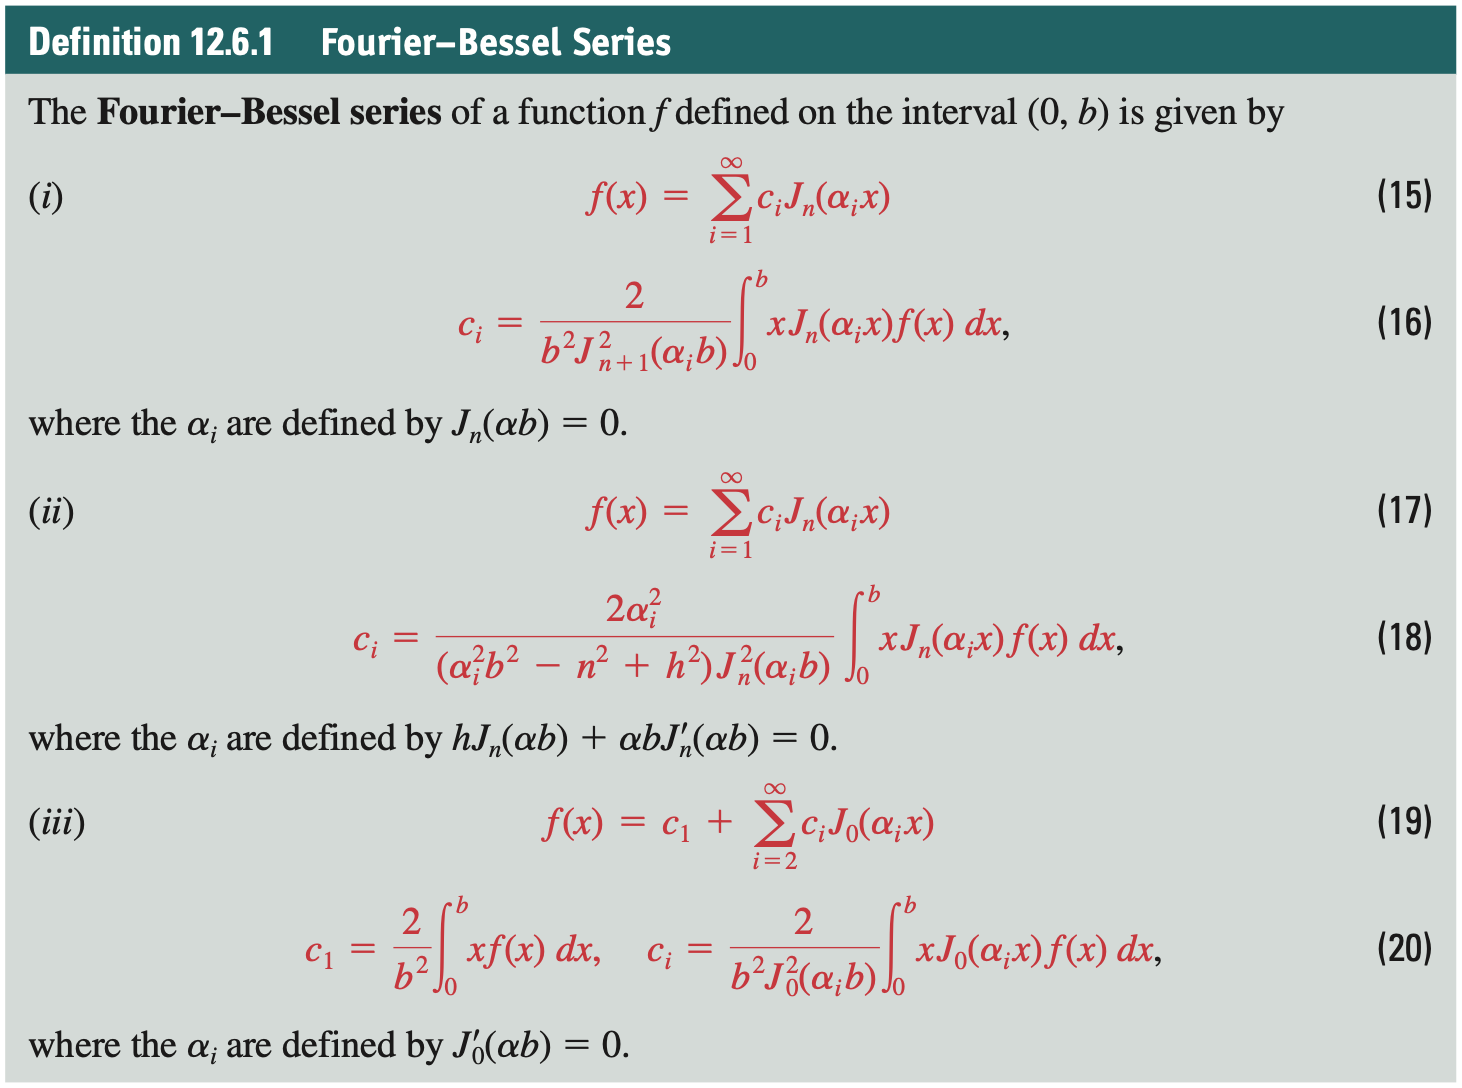
\includegraphics[scale=0.47]{fourier-bessel-series}

\begin{itemize}
  \item The Fourier-Bessel series converges to $f$ where it is continuous and \[\frac{f(x+) + f(x-)}{2}\] where it is discontinuous.
\end{itemize}

\subsubsection{Fourier-Legendre Series}

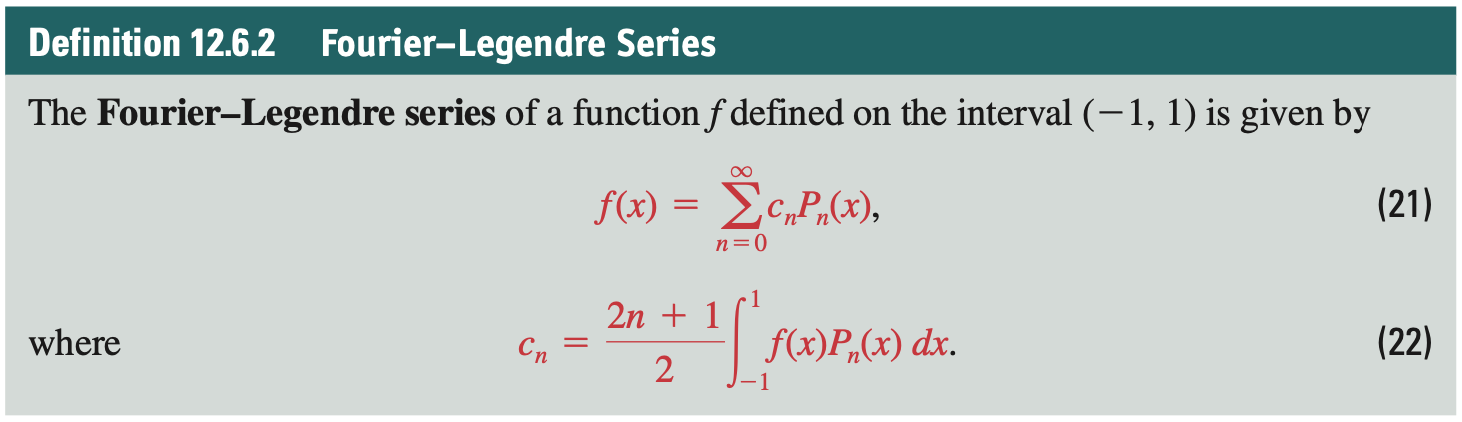
\includegraphics[scale=0.47]{fourier-legendre-series}

\begin{itemize}
  \item The Fourier-Legendre series converges to $f$ where it is continuous and \[\frac{f(x+) + f(x-)}{2}\] where it is discontinuous.
\end{itemize}

\section{Boundary-Value Problems in Rectangular\\Coordinates}

\subsection{Separable Partial Differential Equations}

\begin{itemize}
  \item Like ordinary differential equations (ODEs), partial differential equations (PDEs) can be linear or nonlinear. If the dependent variable and its partial derivatives only appear to the first power, it's a linear PDE.

  \item The general form of a \textbf{linear second-order partial differential equation} is \[A \frac{\partial^2 u}{\partial x^2} + B \frac{\partial^2 u}{\partial x \partial y} + C \frac{\partial^2 u}{\partial y^2} + D \frac{\partial u}{\partial x} + E \frac{\partial u}{\partial y} + F u = G.\] When $G(x, y) = 0$ the equation is said to be \textbf{homogeneous}, otherwise it's \textbf{nonhomogeneous}.

  \item Under the method of \textbf{separation of variables} we assume that the solution of a PDE is a product of functions of each independent variable, e.g. if we seek a solution with independent variables $x$ and $y$ we assume it has the form $u = X(x) Y(y)$. With this assumption it's sometimes possible to reduce the PDE into multiple independent ODEs.

  \item A key step during the process of applying the method of separation of variables is when the equation has been reduced to a form like \[F(X, X', X'') = G(Y, Y', Y'').\] Remembering that $X$ and $Y$ are functions of a single variable, this means that varying $x$ independently of $y$ or vice versa affects one side of the equation but not the other. In order for them to remain equal this means both sides must be constant. This lets us equate each side with a \textbf{separation constant}, giving us an ODE that can be solved on its own.

  \item The \textbf{superposition principle} states that if $u_1, u_2, \ldots, u_n$ are solutions of a homogeneous linear partial differential equation, then the linear combination \[u = c_1 u_1 + c_2 u_2 + \ldots + c_n u_k\] is also a solution.

  \item A linear second-order partial differential equation in two independent variables with constant coefficients \[A \frac{\partial^2 u}{\partial^2 x} + B \frac{\partial^2 u}{\partial x \partial y} + C \frac{\partial^2 y}{\partial y^2} + D \frac{\partial u}{\partial x} + E \frac{\partial u}{\partial y} + F u = G\] can be classified as one of three types:

        \begin{itemize}
          \item \textbf{hyperbolic} if $B^2 - 4 A C > 0$,

          \item \textbf{parabolic} if $B^2 - 4 A C = 0$, and

          \item \textbf{elliptic} if $B^2 - 4 A C < 0$.
        \end{itemize}
\end{itemize}

\end{document}